\chapter{Fonctions Booléennes et circuits logiques}
\section{Fonctions Booléennes}
\subsection{Fonction logique}
Comme précédemment introduit, on peut définir :
\begin{equation}
	F=f(a_0,a_1,\dots,a_{n-1})
\end{equation} 
\hfill où $
\left\{
	\begin{array}{l}
		f = \text{fonction logique (Booléenne)}\\
		a_i= \text{arguments de la fonction } (i=0,\dots,n-1)\\
		F= \text{résultat de l'évaluation}
	\end{array}
\right.
$\\

On peut faire l'analogie avec un système composé de circuits logiques, où les $a_i$ seraient les entrées et $F_i$ les différentes sorties calculées par des fonctions logiques (une fonction logique par sortie, indépendante du reste). De ceci sort la notion de \textit{concurrence}, c'est-à-dire que plusieurs évaluations se font en parallèle.
\section{Modes de représentation}
Rappelons quelques représentations pour une fonction logique :
\begin{itemize}
	\item Tables de Vérité
	\item Expression logique (plusieurs options possibles, certaines plus «belle» que d'autres)
	\item Logigramme
\end{itemize}
\subsection{Tables de Vérité}
Représente la fonction logique de façon unique. Toutes combinaisons des valeurs d'entrée on une valeur de sortie. S'il y a plusieurs sorties, chacune aura sa propre TdV. \\

Ainsi, pour un nombre $n$ d'arguments, la TdV énumérera toutes les combinaisons possibles d'entrées et de sorties. Donc :
\begin{itemize}
	\item TdV constitué de $2^n$ lignes
	\item $2^{2^n}$ fonctions logiques différentes ($0$ ou $1$ pour chaque ligne)
\end{itemize}
À titre informatif:
\begin{figure}[H]
	\centering
	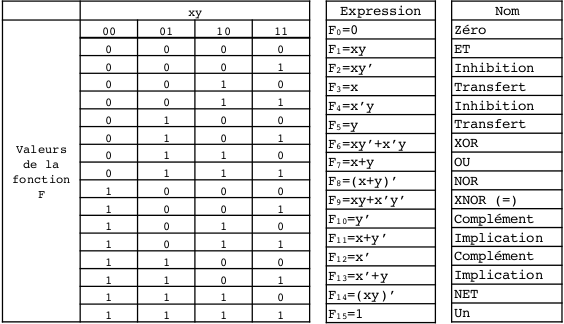
\includegraphics[scale=0.8]{ch3/image1}
\end{figure}

\subsection{Expression algébriques}
À partir de la TdV, on peut définir des expressions algébriques sous 2 formes :
\begin{enumerate}
	\item Forme canonique standard
	\item Forme canonique non-standard
\end{enumerate}
2 expressions différentes (une standard, l'autre non-standard) d'une même TdV sont équivalentes.
\subsubsection{Forme canonique standard}
En procédant comme dans le paragraphe \nameref{subsubsec : TdV->SdP}, nous obtenons une somme de produits dont chaque terme est composé de toutes les variables. Ces termes sont appelés \textbf{Mintermes}. Pour alléger l'écriture de la somme des Mintermes, nous convertissons en décimal chaque combinaison en définissant le \textit{MSB} et le \textit{LSB}.
\begin{figure}[H]
	\centering
	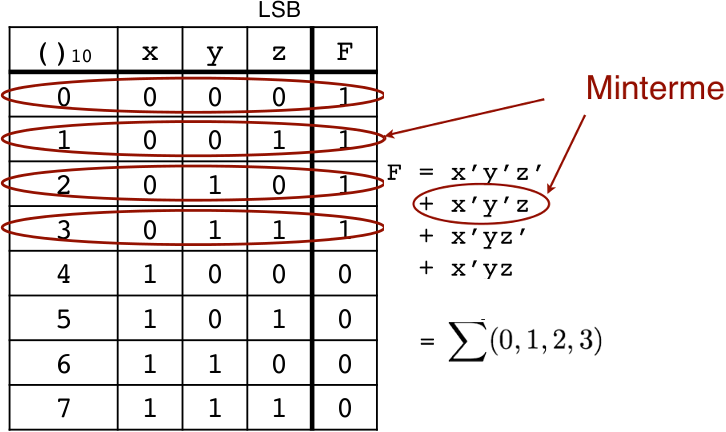
\includegraphics[scale=0.45]{ch3/image2}
\end{figure}


En procédant comme dans le paragraphe \nameref{subsubsec : TdV->PdS}, nous obtenons un produit de sommes dont chaque terme est composé de toutes les variables. Ces termes sont appelés \textbf{Maxtermes}. Même méthode pour la notation abrégée (\danger\ pas $\sum$ mais $\prod$)
\begin{figure}[H]
	\centering
	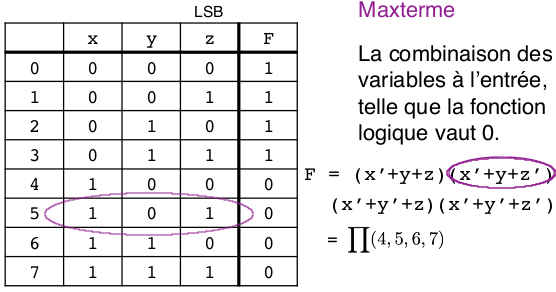
\includegraphics[scale=0.6]{ch3/image3}
\end{figure}
Ainsi, la forme canonique standard s'exprime sous 2 formes: 
\begin{enumerate}
	\item Somme des Mintermes - Forme disjonctive normale
	\begin{center}
		\textbf{Somme logique (OU) des termes produits (ET) pour lesquels la fonction logique a pour valeur «1»}
	\end{center}
	\item Produit des Maxtermes - Forme conjonctive normale
	\begin{center}
		\textbf{Produit logique (ET) des termes sommées (OU) pour lesquels la fonction logique a pour valeur «0»}
	\end{center}
\end{enumerate}
\subsubsection{Forme canonique non-standard}
Le but est de simplifier l'expression de la fonction logique. Par exemple, la fonction logique précédente pouvait se résumer à $F=x'$.\\
On peut réduire:
\begin{itemize}
	\item le nombre de termes dans la somme ou le produit
	\item chaque terme de la somme ou le produit
\end{itemize}
Après simplification, la fonction logique se compose de termes appelés \textbf{monômes} (ne possédant pas toutes les variables).\\

Pour repasser sous forme canonique, rien de très compliqué
\begin{itemize}
	\item Minterme
	\begin{equation}
		xy'=xy'\cdot 1=xy'\cdot(z+z')=xy'z+xy'z'
	\end{equation}
	\item Maxterme
	\begin{equation}
		x+y'=x+y'+0=x+y'+zz'=(x+y'+z)\cdot(x+y'+z')
	\end{equation}
\end{itemize}
\section{Simplification}
La simplification des fonctions logiques comportent certains intérêt comme:
\begin{itemize}
	\item $\searrow$ du nombre de portes logiques dans le circuit
	\item $\nearrow$ de la vitesse de commutation (moins de transistors, moins de portes en séries)
	\item $searrow$ du prix
\end{itemize}
Il y a néanmoins des problèmes avec la simplification via les axiomes et les théorèmes, nous n'avons aucune certitude que 
\begin{itemize}
	\item l'expression est simplifiable
	\item l'expression d'arrivée est la plus simple
\end{itemize} 
\section{Logique à 2 et à plusieurs niveaux}
Toute fonction logique dans un logigramme est un plan de portes ET avec une porte OU au bout. De la peut sortir la notion de \textbf{niveau}. On définit le délai comme \textit{le délai de 2 plans de portes, quelque soit la fonction}
\begin{figure}[H]
	\centering
	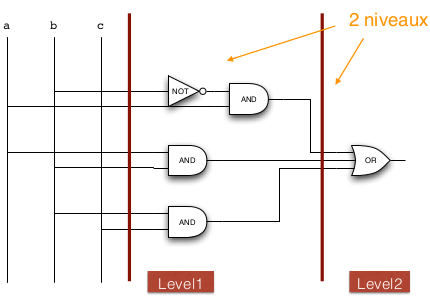
\includegraphics[scale=0.7]{ch3/image4}
\end{figure}
Mais comment une SdP évolue avec la complexité croissante de la fonction logique (lorsque le nombre d'entrées augmente)?\\

En théorie: uniquement la surface.\\
En pratique:
\begin{itemize}
	\item chaque porte sera plus grande (capacitance $\nearrow$, impact sur le délai et la puissance)
	\item $\nearrow$ longueur des fils (délais)
\end{itemize}
\begin{figure}[H]
	\centering
	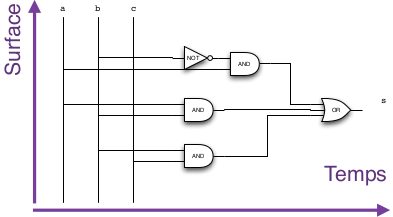
\includegraphics[scale=0.7]{ch3/image5}
\end{figure}
Il faudra donc jouer sur ces 2 paramètres (surfaces/délais) en sachant que nous ne pourrons pas gagner sur tous les plans. Cette optimisation fera partie de l'\textit{optimisation des circuits logiques} (chapitre important)
\subsection{Expansion de Boole (Shannon)}
Une fonction logique $F(x_i),\quad i=0,\dots,n$ peut être représentée comme:
\begin{align}
	F(x_i) &= x_1F_1(1,x_2,\dots,x_n)+x_1'F_1(0,x_2,\dots,x_n)\\
	&= (x_1+F_1(x_j))(x_1'+F_1(x_j))\\
	&= x_jF_1(x_j)+x_j'F_1(x_j)\qquad i=0,\dots,n\quad j=1,\dots,n
\end{align}
Ainsi, toute fonction logique peut être diviser en 2 fonctions logiques (une pour $x$, l'autre pour $x'$). Il y a \textbf{factorisation de la fonction logique}.\\

De cette manière, les 2 fonctions résultantes peuvent être évaluées séparément (en parallèle) et fusionner les résultats. Il en résulte des porte plus simples ($\searrow$ nombre d'arguments), donc un calcul qui explose en surface peut être décomposé en temps ($\searrow$ surface, $\nearrow$ niveaux/délais).